

Click on the  icon of  \texttt{\getsoftwarename{}} to open the application.
Click the "+" button to add a soil layer (\Cref{fig:addLayer}). Click several times to add more layers.

\begin{figure}[!htbp]
  \centering {
    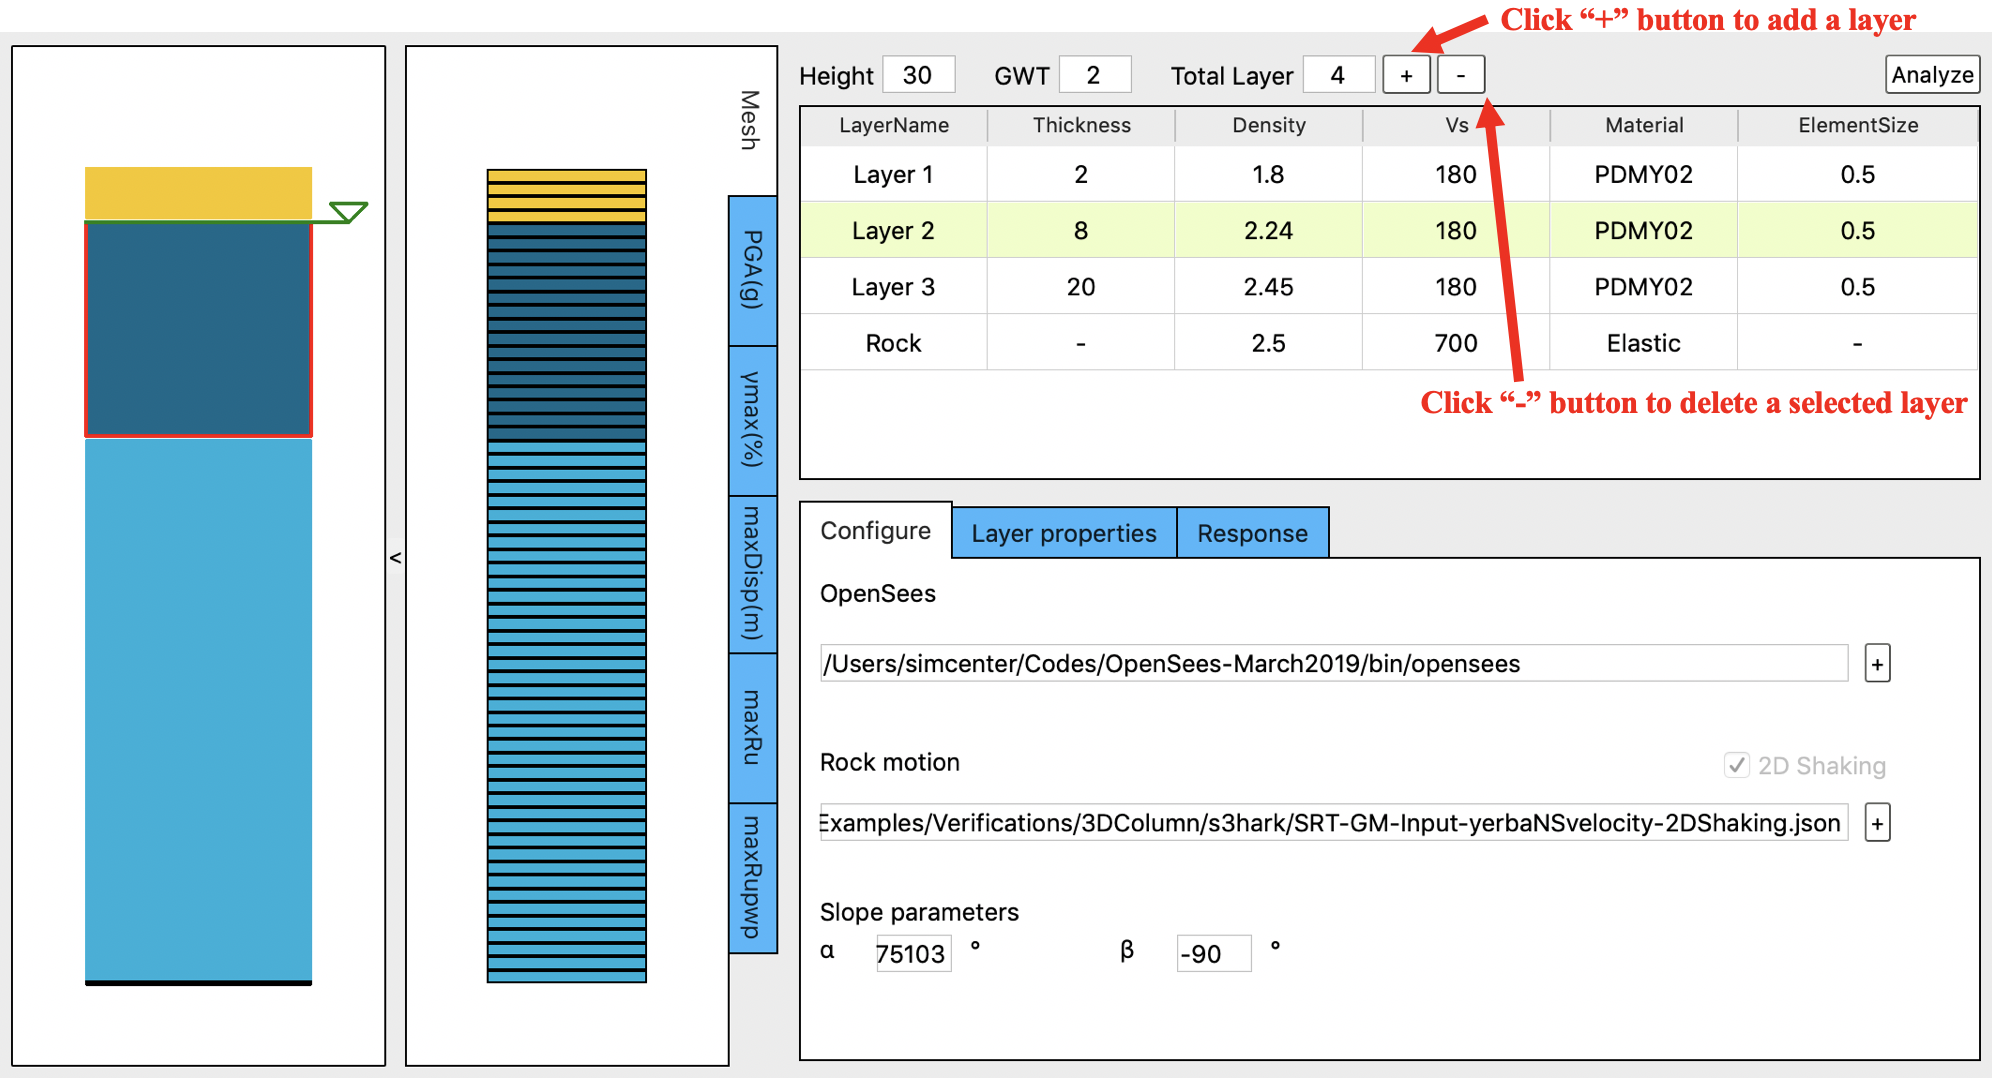
\includegraphics[width=0.9\textwidth]
    {installation/figures/addLayer.png} }
  \caption{Adding soil layers}
  \label{fig:addLayer}
\end{figure}


Click on the configure tab to show configurations options. 
Under the "OpenSees" label, type the path of OpenSees executable. 
You can also select the executable from your local computer by clicking on the "+" button on the right of the input area (\Cref{fig:addOpenSees}).

Under the "Rock motion" label, type the path of a ground motion file. 
You can also select the file from your local computer by clicking on the "+" button on the right of the input area (\Cref{fig:addOpenSees}).

\begin{figure}[!htbp]
  \centering {
    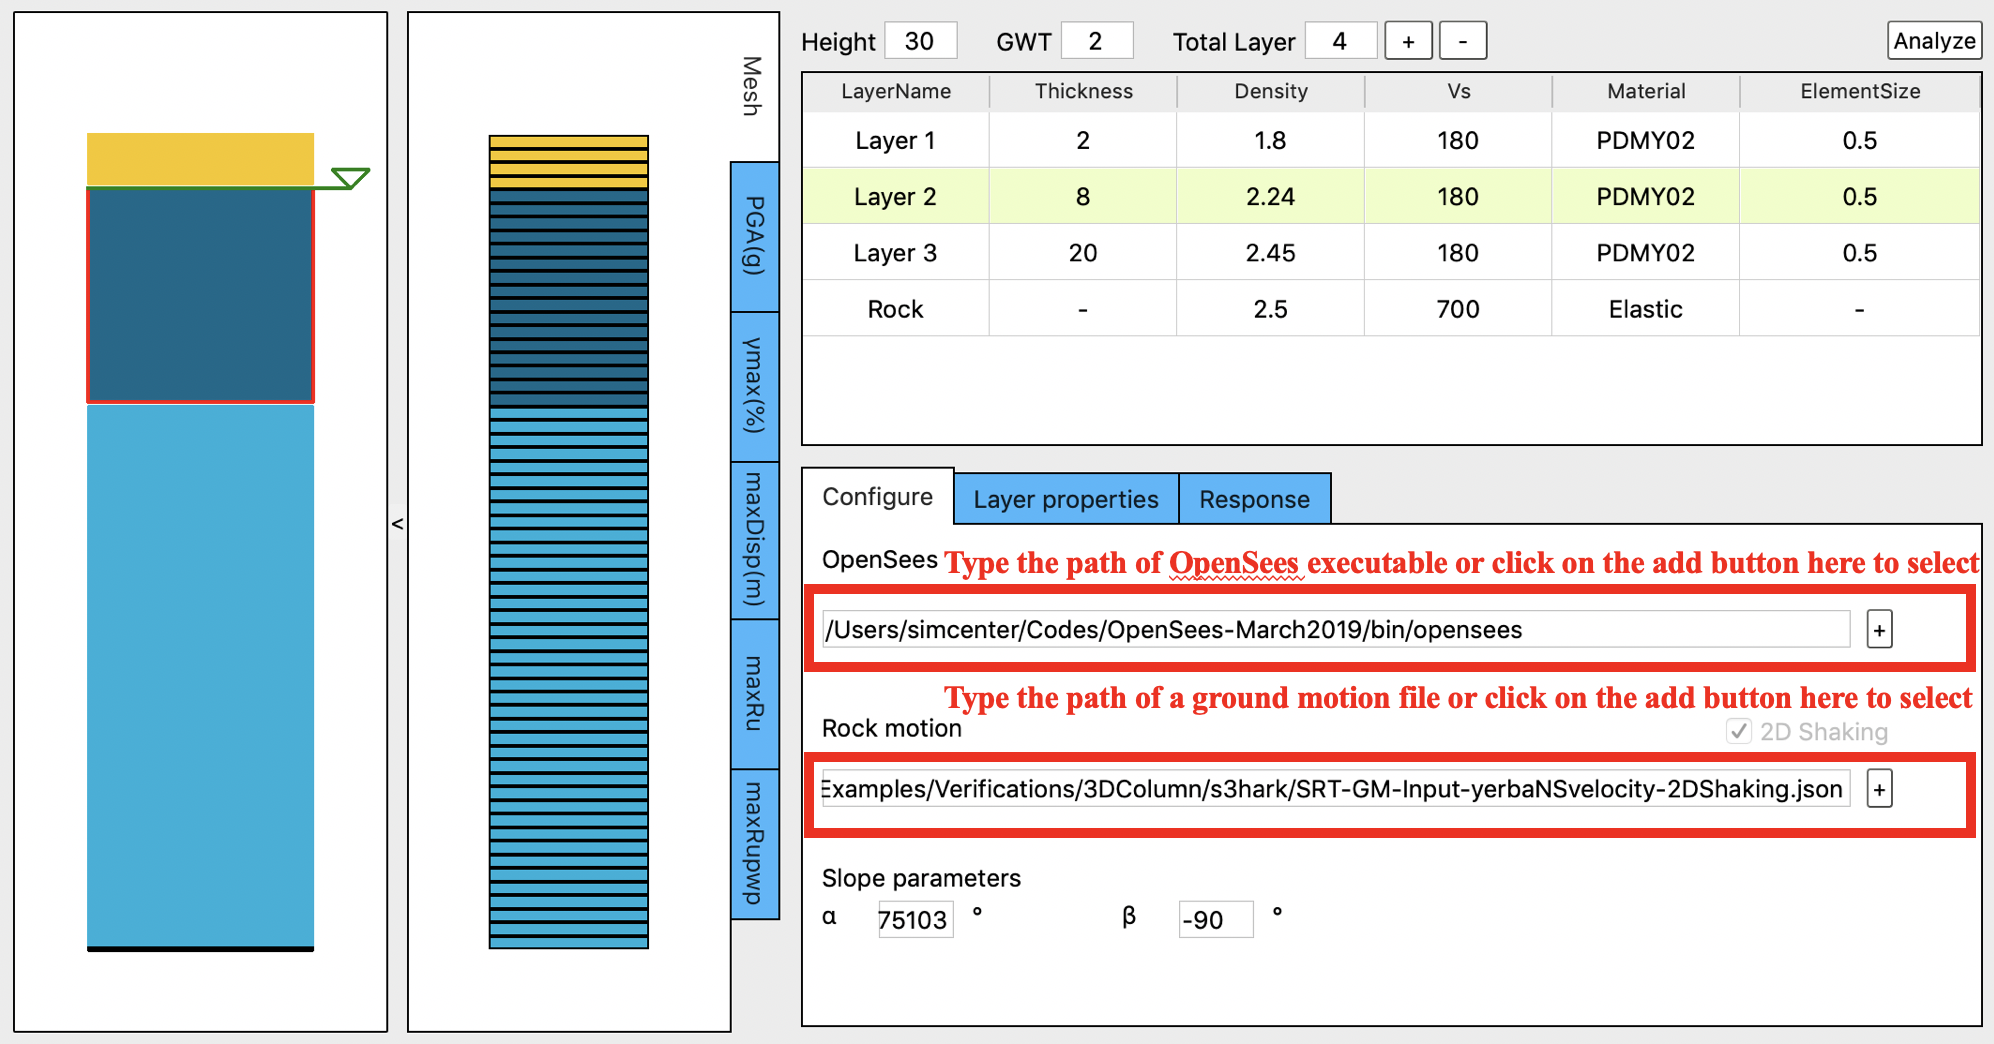
\includegraphics[width=0.9\textwidth]
    {installation/figures/addOpenSees.png} }
  \caption{Adding OpenSees path and rock motion file}
  \label{fig:addOpenSees}
\end{figure}


\begin{figure}[!htbp]
  \centering {
    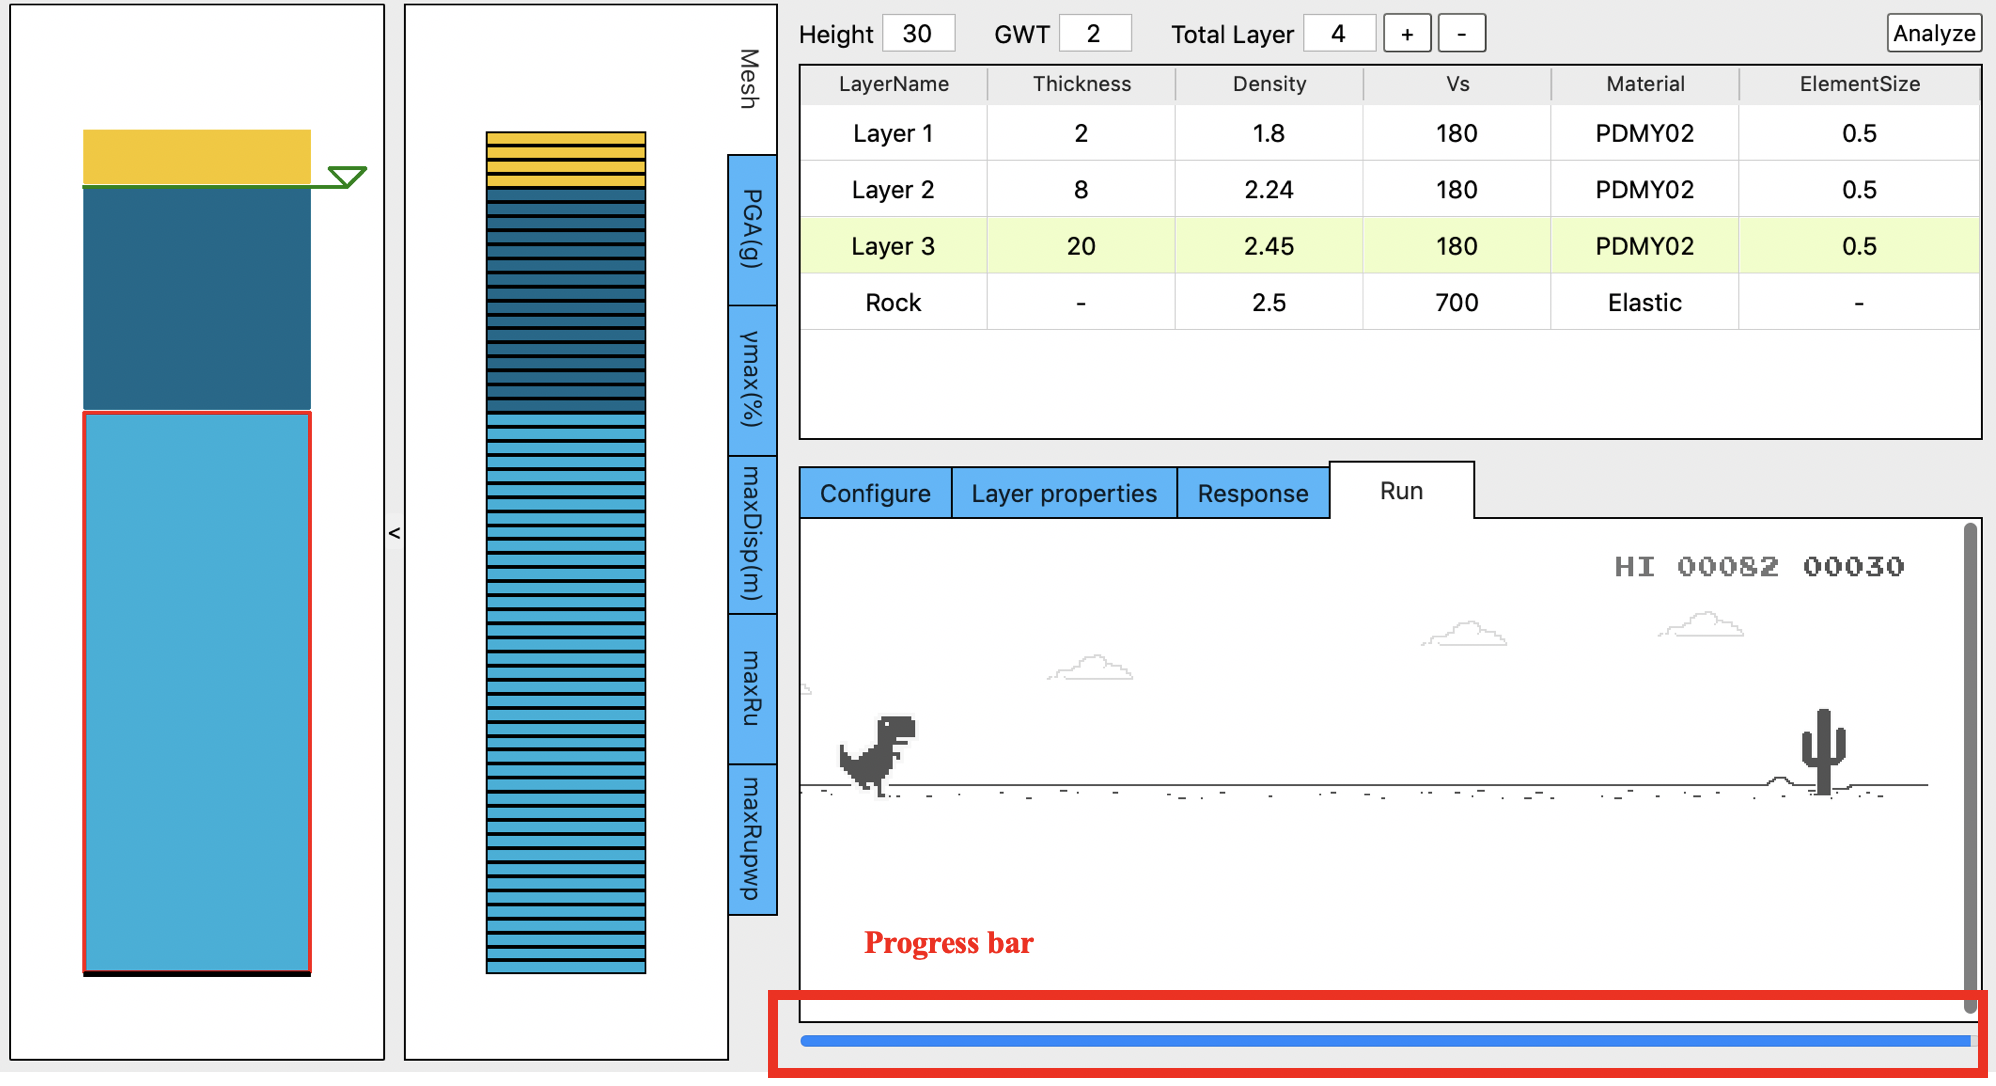
\includegraphics[width=0.9\textwidth]
    {installation/figures/progress.png} }
  \caption{Simulation progress }
  \label{fig:progress}
\end{figure}

Click on the "Analyze" button to run the finite element analysis.
If the soil layers are added successfully, OpenSees path is correct and the rock motion file is correct,
you will see a progress bar (\Cref{fig:prpgress}) displayed at the bottom of the right hand side of the app, which shows the percentage of steps performed. 

\begin{figure}[!htbp]
  \centering {
    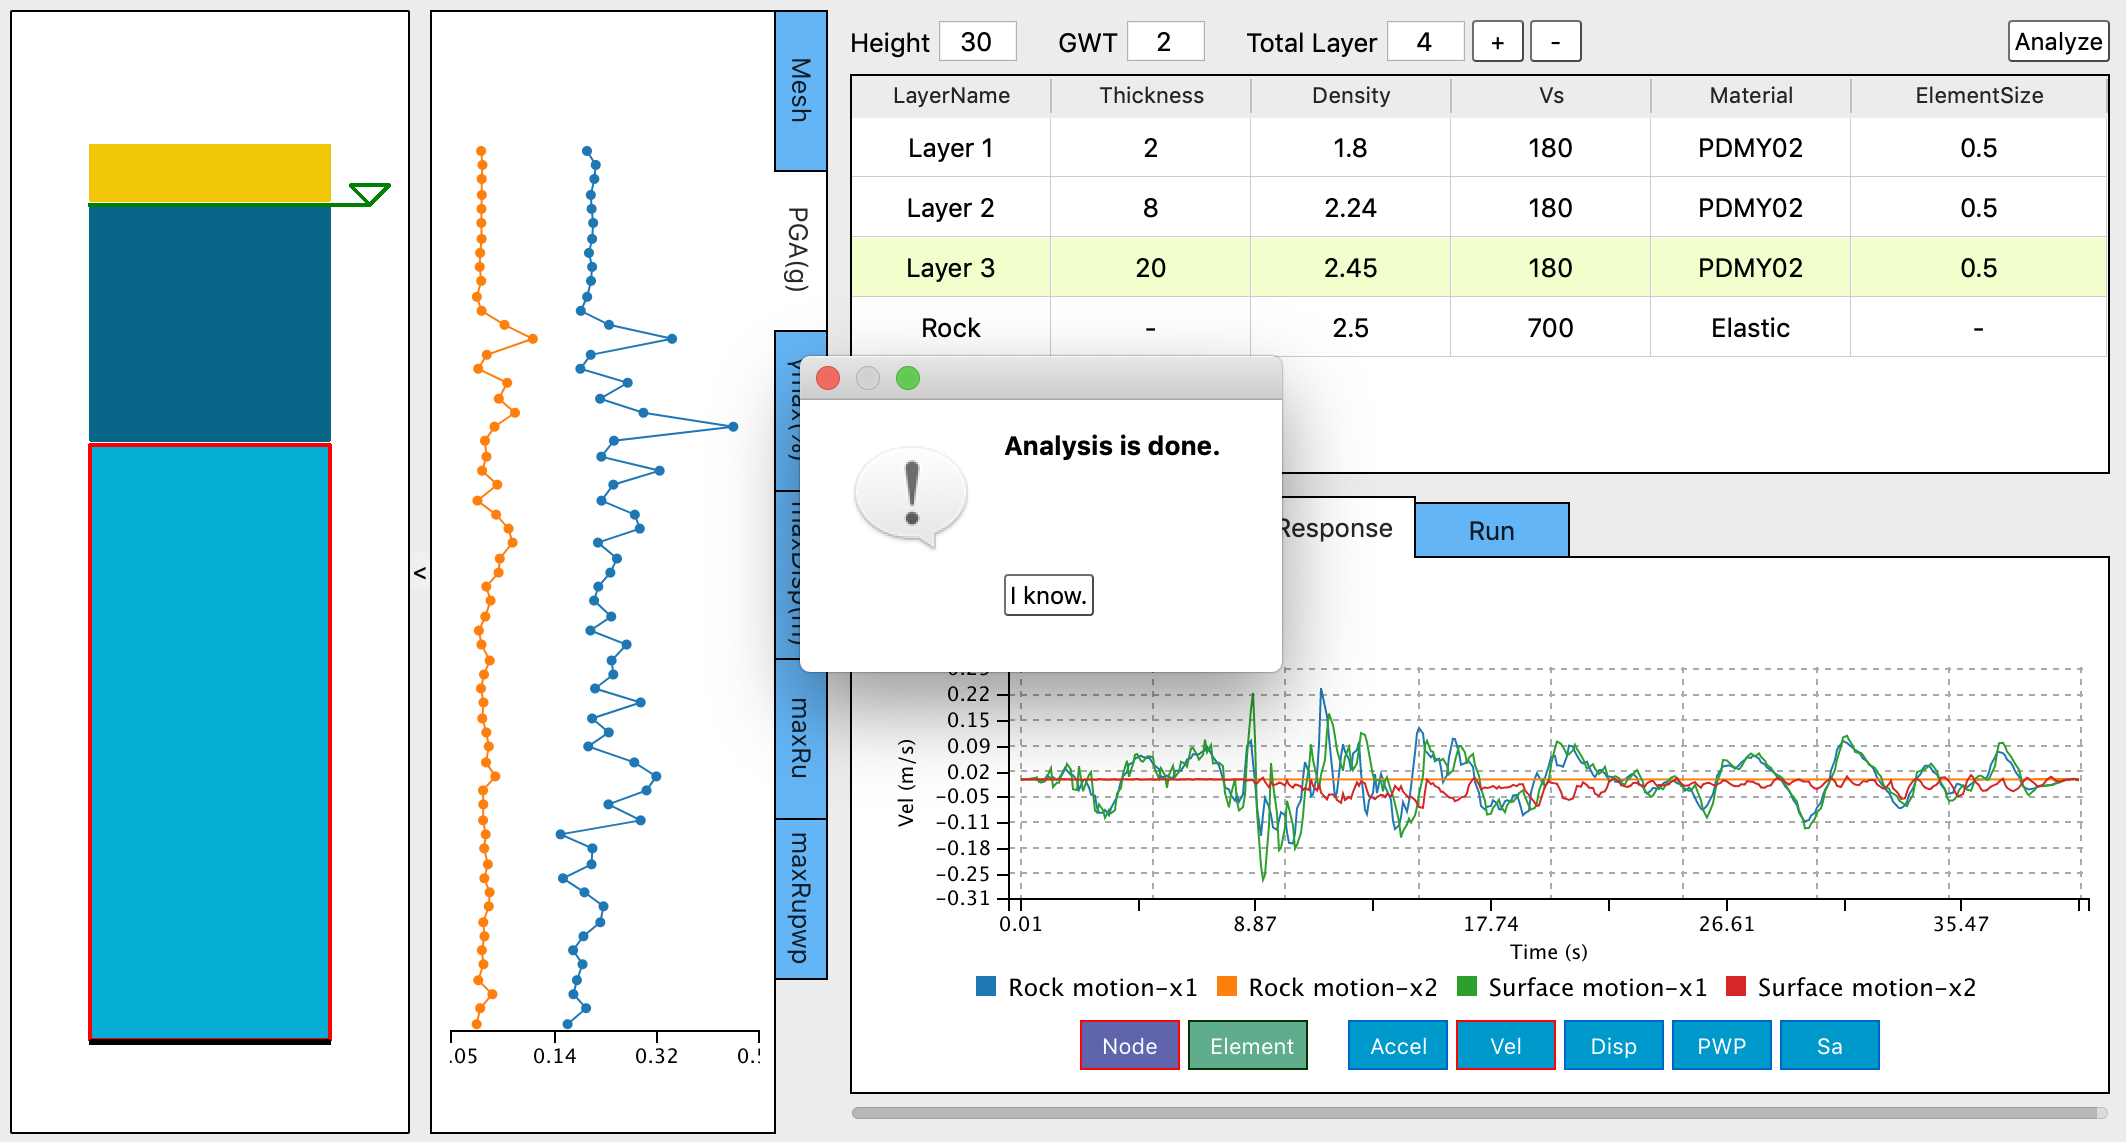
\includegraphics[width=0.9\textwidth]
    {installation/figures/done.png} }
  \caption{Analysis is done }
  \label{fig:done}
\end{figure}

Once the simulation is done, the "Response" tab and the "PGA(g)" profile plot will be displayed.
At the same time, 
a pop up window showing "The analysis is done." will show up.
And when you click "I know.", the progress bar will disappear.
